% -*- mode: LaTeX; coding: utf-8; -*-

\chapter{Web 2.0 teknologiat}

\section{Yleistä}

Internet on aina ollut ja tulee aina olemaan vihamielinen paikka, jossa sivustolla vierailevan motiiveja sivustoa ja palvelua kohtaan on mahdoton ennustaa. Tästä syystä 
useimmat kehittäjät ja ylläpitäjät ovat noudattaneet periaatetta, että kehenkään ei voi täysin luottaa. Sivustojen ja palveluiden kehittyessä entistä monimutkaisemmiksi
Web 2.0:n myötä, on tämän periaatteen noudattaminen noussut entistä tärkeämmäksi. Tämä ei tarkoita sitä, että Web 2.0:n takana olevat teknologiat olisivat normaalia 
heikompia tai että ne sisältäisivät helposti hyödynnettäviä haavoittuvaisuuksia. Web 2.0 mahdollistaa vain aikaisempaa joustavamman alustan toteuttaa interaktiivisia ja
normaaleja työpöytäsovelluksia muistuttavia palveluita, joita käyttäjät voivat ajaa suoraan web-selaimesta. Varsinainen ongelma piilee siinä, että tällaiset palvelut ovat 
aikaisempaa monimutkaisempia toteuttaa. Niissä hyödynnetään useita eri teknologioita ja rajapintoja, jonka johdosta mahdollisuus tehdä virheitä kasvaa verrattaessa
vanhoihin ratkaisuihin. Itse käytetyt teknologiat eivät siis ole syynä heikentyneeseen tietoturvatasoon, vaan syynä on kehittäjien huolimattomuus ja/tai tietämättömyys 
niistä mahdollisuuksista, joita huonosti koodatut palvelut avaavat hyökkääjille. Tämän luvun tarkoitus onkin lyhyesti esitellä tärkeimmät Web 2.0:n takana olevat teknologiat, 
ja tuoda esille osa niistä riskeistä, joita huonosti toteutetut sovellukset voivat aiheuttavat. 

\section {AJAX}

Jos jokin Web 2.0 teknologiosta halutaan nostaa kehitystä eniten eteenpäin vieväksi voimaksi, niin vahvin ehdokas tähän on AJAX.  Asynchronous JavaScript and XML (lyh. AJAX)
itsessään ei ole mikään yksi tietty teknologia, vaan se on usean eri teknologian yhdistelmä, joita käyttämällä web-sovellukset pystytään muuttamaan nopeasti reagoiviksi
ja käyttökokemukset tuomaan lähemmäksi perinteisiä työpöytäsovelluksia \cite{AJAX}. AJAX koostuu seuraavista teknologioista:

\begin{itemize}
\item HTML ja CSS rakentavat web-selaimella näytettävän sivun.
\item DOM mahdollistaa käytön aikaisen dynaamisen sisällön tuottamisen.
\item XML ja Extensible Stylesheet Language Transformation (lyh. XSLT) mahdollistavat kerrosten välisen tiedonsiirron.
\item JavaScript helpottaa eri komponenttien integroimisen sekä näiden ohjelmoimisen.
\item XMLHttpRequest (lyh. XHR) objekti helpottaa serverien välistä kommunikointia \cite{WEB2b}.
\end{itemize}

Suurin AJAXin tuoma muutos perinteisiin web-sivuihin on mahdollisuus päivittää sivun sisältöä asynkronisesti. Yksinkertaistettuna tämä tarkoittaa sitä, että sivun sisällöstä
pystytään päivittämään ainoastaan halutut osat käyttäen XHR-kanavia. Aikaisemmin tällainen ei ole ollut mahdollista, sillä vanhat web-sivut ovat toimineet pelkästään synkronisesti, jolloin 
erillisiä kutsuja ei ole voitu tehdä. Tämän takia koko sivu on täytynyt päivittää kerralla. Tämä on hidastanut käyttökokemusta, sillä päivityksen nopeus on riippunut siitä, 
kuinka nopeasti palvelin ja selain ovat pystynyt päivittämään sivut. XHR sisältää kaikki perinteiset HTTP metodit mukaanlukien GET, POST, HEAD ja DELETE, joten sen avulla pystytään suorittamaan
kaikki yleisimmät käyttäjän toiminnot \cite{WEB2}. Kuvassa \ref{synkroninen} on esitetty tilanne, jossa sama palvelu on toteutettu käyttäen synkronisia ja asynkronisia 
kutsuja. Kuvasta näkee, että Web 2.0 mahdollistaa useamman yhtäaikaisen kutsun tekemisen, jolloin myös palvelun käyttäminen on nopeampaa.

\begin{figure}[htp]
\centering
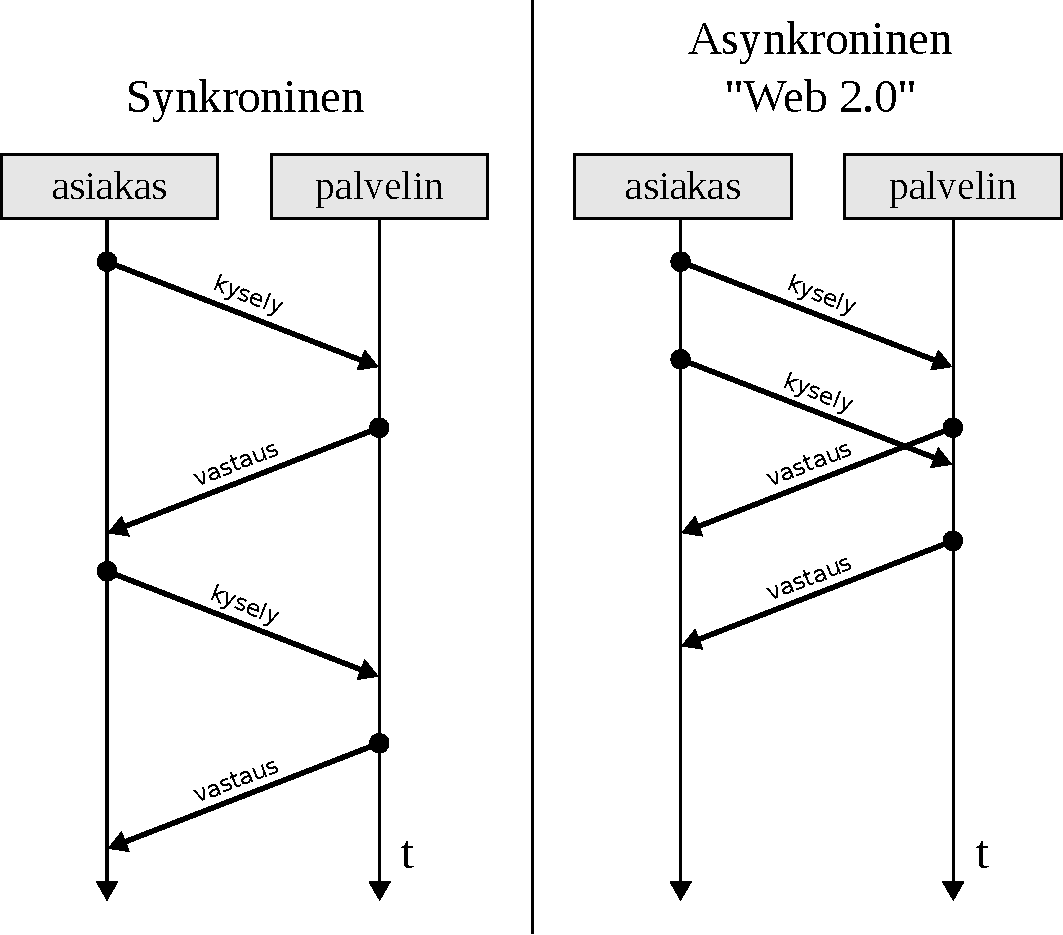
\includegraphics[width=12cm]{pics/synkroninen.pdf}
\caption{Synkroninen ja asynkroninen kommunikointi}
\label{synkroninen}
\end{figure}

AJAXiin kohdistuvat hyökkäykset eivät eroa kauheasti vanhoista murtautumismenetelmistä. Hyökkääjät pyrkivät edelleen hyödyntämään syötteen puutteellista suodattamista, muokkaamaan ulostulevaa
dataa, murtamaan salauksia ja hankkimaan istuntonkohtaisia tietoja esimerkiksi evästeitä varastamalla. Se, mikä erottaa AJAXin vanhemmista tekniikoista ja tekee siitä samalla kiinnostavan
kohteen hyökkääjille, on sen tapa luottaa entistä enemmän asiakaspuolen JavaScripteihin. Asiakaspuoleen ei voida koskaan luottaa, ja JavaScriptien huolimaton käyttö avaa hyökkääjille monia
tapoja murtaa asetetut suojaukset. Nämäkään eivät ole uusia asioita, mutta kiinnostuksen siirtyessä AJAXiin, ovat myös hyökkääjät alkaneet kiinnittämään näihin enemmän huomiota \cite{AJAX}.
Monet käytetyistä AJAX-ympäristöistä sisältävät myös eriasteisia tietoturvariskejä, joita hyökkääjät voivat hyödyntää \cite{JSH}.

\subsection{JavaScript}

JavaScript on Netscapen suunnittelema skriptikieli, joka tunnettiin aluksi nimellä LiveScript. Sun Microsystemsin kehittämän Java-ohjelmointikielen yleistyessä Netscape päättii muuttaa 
sen nimen JavaScriptiksi, toivoen sen käytön yleistyvän Javan menestyksen myötä. JavaScriptillä kirjoitetut skriptit tunnistaa HTML:n elementistä <script>, ja toimiakseen se tarvitsee ympäristön,
josta löytyy tuki JavaScriptille. JavaScript on tehokas työkalu, joka  mahdollistaa monen muun toiminnon ohella mm. dynaamisten web-sivujen tekemisen, viestien kirjoittamisen selaimen 
tilariville, uusien ikkunoiden avaamisen ja interaktiivisten lomakkeiden luomisen. Skriptien toiminta rajoittuu kuitenkin web-selaimen toimintoihin, eikä sitä käyttäen voida esimerkiksi 
kirjoittaa levylle ja levyn lukeminen rajoittuu pelkästään evästeisiin \cite{JavaScript}. Näistä rajoituksista huolimatta JavaScript mahdollistaa erittäin monipuolisten toimintojen 
toteuttamisen web-ympäristössä.

Suurin osa web-sivuilla olevista skripteistä toimii siten, että ne ladataan aluksi käyttäjän koneelle, jonka jälkeen ne suoritetaan selaimessa. Skriptit sijaitsevat käyttäjien 
koneilla, joten toimintaperiaatten selvittäminen ei ole hyökkääjälle vaikeaa. Asiaa pystytään kuitenkin vaikeuttamaan muutamalla eri tavalla. Näistä yksinkertaisin on poistaa koodista
kommentointi ja tyhjät rivivälit, jolloin koodin lukeminen on vaikeampaa. Seuraava askel on koodin muuttujien ja objektien uudelleennimeäminen, jolloin hyökkääjän on vaikeampi päätellä näistä
skriptin toimintaperiaate. Nimet voidaan muuttaa esimerkiksi binäärikoodiksi, mutta tämän haittapuolena on tiedoston koon kasvaminen. Nämä keinot ovat kuitenkin vain hidasteita osaavalle 
hyökkääjälle. Paras keino sisällön peittämiselle on käyttää jonkinlaista salausmenetelmää, ja osa selaimista sisältääkin suoraan tällaisen mahdollisuuden. Tämäkään ei takaa suojaa täydellistä
turvaa, mutta pieni suojaus on kuitenkin parempi kuin ei suojausta ollenkaan \cite{AJAX}.

Koneelle ladatut skriptit ajetaan oletuksena hyvin rajatussa tilassa, jossa niillä on pääsy vain kyseistä sivua käsittävään dataan tai siihen hyvin läheisesti kuuluviin dokumentteihin. 
JavaScript noudattaa myös jo edellisessä kappaleessa esitetty \emph{saman alkuperän} periaatetta, joka rajoittaa skriptien toimimisen vain sen domainin sisällä, josta sitä on kutsuttu.  
Tällä tavoin estetään hyökkäyksen tekeminen käyttäen toiselta sivulta ladattua haitallista skriptiä, jonka avulla voitaisiin esimerkiksi varastaa evästeitä ja urkkia näppäimistön painallukset.
Aikaisemmin selaimet ovat sallineet joitain poikkeuksia tähän periaatteeseen, mutta tietoturvasyistä nämä on kuitenkin poistettu. Liian tiukat tietoturvasäännöt eivät kuitenkaan toimi
nykyaikaisten web-palveluiden kanssa, ja tästä syystä \emph{saman alkuperän} periaatetta on mahdollista löysentää. Esimerkiksi ulkoiset linkit, jotka osoittavat toisella sivustolla olevaan
skriptiin, ohittavat \emph{saman alkuperän}, sillä vaikka itse skripti sijaitsee toisella sivustolla niin se lasketaan kuuluvan siihen sivustoon, josta kutsu tehtiin. Näin ollen 
kutsutulla skriptillä on pääsy sellaisiin evästeisiin ja tiedostoihin, joihin sillä ei välttämättä tarvitsisi olla oikeuksia. Sivustojen ja palveluiden hakiessa tulevaisuudesa
entistä useammasta osoitteesta tarvittavia resursseja, voi tämä aiheuttaa riskitilanteita, jos joku näistä resursseista on altistettu hyökkäykselle \cite{AJAX}.

\subsection{AJAXiin liittyvät tietoturvariskit}

Koska AJAXin toiminta perustuu hyvin pitkälti JavaScriptin varaan niin on itsestään selvää, että hyökkääjät pyrkivät hyödyntämään tätä seikkaa. Se tarjoaa hyökkääjille tehokkaan työkalun,
jonka avulla käyttäjän asettamaa luottamusta voidaan väärinkäyttää. Asiaa ei auta se, että suurin osa sivustoista on jollakin asteella alttiina XSS-hyökkäyksille \cite{WEB2c} johtuen huonosti
toteutetusta syötteen suodatuksesta. Asetettuja suodatuksia pystytään myös kiertämään käyttäen esimerkiksi kuvalinkkejä ja erilaisia tageja, joiden avulla ajettava skripti voidaan 
hukuttaa muun syötteen joukkoon. Juuri tästä syystä pelkästään tiettyjen merkkijonojen suodattaminen ei takaa suojaa JavaScript-pohjaisilta hyökkäyksiltä. Tehokkain ja yksinkertaisin keino
onkin muuttaa kaikki tagit HTML merkeiksi, jolloin esimerkiksi < merkistä tulee \emph{&lt;} ja > merkistä \emph{&gt;}. Monet ympäristöt mahdollistavat myös suoraan HTML-elementtien
poistamisen käyttäjien jättämistä viesteistä \cite{AJAX}.

Kasvaneella JavaScriptin käytöllä on suora vaikutus myös XSS-hyökkäysten yleistymiseen. JavaScript pääsee helposti evästeisiin käsiksi käyttäen \emph{document.cookie} kutsua, ja vaikka sen 
käyttö on rajoitettu ainoastaan sen domainin evästeeseen, josta kutsu on tehty, voidaan tämä rajoitus ohittaa melko helposti. Hyökkääjälle riittää, että käyttäjä vierailee esimerkiksi sellaisessa
foorumissa tai blogissa, jossa viesteissä sallitaan XHTML:n käyttö. Tämä mahdollistaa haitallisten skriptien lähettämisen sivustolle ja pahaa aavistamaton käyttäjä, joka vierailee tällä
sivulla, joutuu tietämättään hyökkäyksen kohteeksi. Yksi tapa suojautua evästeiden varastamiselta on käyttää HTTP-Only -evästeitä, jolloin asiakaspuolen evästeitä ei pystytä lukemaan. Näiden
evästeiden tukeminen on kuitenkin selainkohtaista, joten tämä ratkaisu ei aina välttämättä ole mahdollista toteuttaa. XSS-hyökkäykset eivät myöskään rajoitu pelkästään evästeiden varastamiseen,
ja yhtä helposti hyökkääjä voi esimerkiksi luoda skriptin, joka lukee näppäimistön painallukset ja lähettää ne haluttuun osoitteeseen. HTTP-Only evästeiden käyttö ei myöskään täysin suojaa 
evästeitä, jos käytetään XHR-kutsuja. Tällöin hyökkääjän on mahdollista lukea suoraan otsaketiedoista asetettuja arvoja, jos hyökkääjä onnistuu kaappaamaan XHR objekteja. Jotkut XHR-objekteihin
liittyvät haavoittuvuudet ovat myös niin syvällä XHMLHttpRequest-objekteissa, että kaikki nykyisin käytössä olevat toteutukset ovat niille jossain määrin vielä alttiina. Kaapattujen XHR-objektien 
tunnistaminen ei myöskään vielä ole mahdollista \cite{AJAX}. Näistä syistä johtuen AJAX tarjoaa nyt ja tulevaisuudessa hyökkääjille monia mahdollisuuksia murtaa asetettuja suojauksia.

Yksi yleisimmistä AJAXissa käytetyistä dataformaateista on JavaScript Object Notationt (lyh. JSON), joka on kielestä riippumaton ja näin ollen useimmat palvelimella käytetyistä kielistä 
pystyvät lukemaan sen sisällön. Se on rakenteeltaan hyvin kevyt, ja se koostuu kahdesta eri tietotyypistä: objekteista ja taulukoista \cite{JSON}. Formaatin heikkous piilee siinä, että 
taulukko itsessään on validi JavaScript-syöte, jonka sisältö on mahdollista kaapata \cite{AJAX}. Termi \emph{JavaScript Hijacking} kuvaa tällaista tilannetta, jossa hyökkääjä ohittaa 
\emph{saman alkuperän} periaatteen silloin, kun JavaScriptiä käytetään arkaluontoisen tiedon lähettämiseen. Aiheesta tehdyn tutkimuksen \cite{JSH} mukaan lähes jokainen käytetty AJAX-ympäristö
on alttiina tällaisilla hyökkäyksille. Käyttäen CSRF-hyökkäystä hyökkääjä pystyy väärinkäyttämään JSON-formaattia, ja varastamaan sekä muokkaamaan toiselle sivustolle lähetettäviä paketteja. 
Tälläinen hyökkäys voidaan toteuttaa useilla eri tavoilla mukaanlukien käyttäen script-elementtiä, ja koska pyyntö tulee selaimen luottamasta lähteestä, voidaan tällä tavoin ohittaa esimerkiksi 
SSL-suojaus \cite{AJAX}. Suojautuminen tämän tyyppisiltä hyökkäyksiltä voidaan toteuttaa monella eri tapaa, ja paras tulos saadaan yhdistelemällä näitä. Koska CSRF-hyökkäyksessä hyökkääjä joutuu 
toimimaan osittain  sokeasti, voidaan jokaiseen pyyntöön lisätä parametri, jota hyökkääjän on vaikea arvata. Palvelin voidaan myös asettaa tarkistamaan HTTP Referer-kenttä, jolla voidaan varmistaa, 
että pyyntö tulee sallitulta taholta, vaikkakin Referer-kentän sisältö voidaan helposti muuttaa. Toinen tapa on muokata vastaanottopäässä paketteja siten, että hyökkääjä ei pysty ajamaan lähettämissään 
pyynnöissä skriptejä \cite{JSH}

\section{Flash}

Ajaxin ohella Macromedian suunnittelema ja nykyisin Adoben kehittämä Flash on ollut yksi niistä kantavista tekniikoista, joita käyttämällä YouTuben ja MySpacen kaltaiset menestyspalvelut ovat olleet 
mahdollisia toteuttaa. Flashia käyttämällä kehittäjät ovat jo pitkään pystyneet luomaan interaktiivista ja rikasta web-sisältöä yksinkertaisista animaatioista aina monimutkaisiin peleihin ja
valikoihin asti. Suurin osa web-sivustoilla olevista mainoksista on myös toteutettu käyttäen Flashia. Näistä syistä johtuen Flash Player on yksi ohjelmistoalan de facto-alustoista, jonka käyttöaste 
yritys- ja kuluttajapuolella on lähes 100 prosenttia \cite{Flash}. 

Flashin sisältämä ActionScript-skriptikieli muistuttaa läheisesti JavaScriptiä, ja sitä käyttäen on mahdollista mm. luoda uusia TCP-yhteyksiä, ajaa JavaScriptiä selaimessa ja luoda sallittuihin 
domaineihin HTTP-pyyntöjä. Flashin käyttämä tietoturvamalli noudattaa paljolti saman alkuperän periaatetta, jolla rajoitetaan eri domaineissa sijaitsevien sovellusten kommunikointia. Domainien
välinen kommunikointi on kuitenkin sallittua, ja käytetty tietoturvapolitiikka luetaan tähän tarkoitetusta XML-tiedostosta. Tämä XML-tiedosto sijaitsee usein domainin juuressa, ja se sisältää ne 
domainit, jotka saavat olla siihen yhteydessä. Osa Flashiin kohdistuvista hyökkäyksistä pyrkiikin muokkaamaan tämän tiedoston sisältöä siten, että kohde sallisi yhteydet myös hyökkääjän käyttämästä
osoitteesta. Tämä voidaan toteuttaa esimerkiksi käyttämällä vihamielistä RSS-syötettä tai luomalla tiedosto, joka sisältää uuden XML-tiedoston. Yksi tällaisista hyökkäyksistä on Stefan Esserin 
luoma GIF-tiedosto, jonka kommenttiin on piilotettu uusi tietoturvapolitiikka. Hyökkääjälle riittää, että kohdekone vain mahdollistaa tiedoston lataamisen palvelimelle, jonka jälkeen vanha 
sisältö voidaan korvata GIF-tiedostoon piilotetulla \cite{WEB2}. 

Perimmäinen syy sille, miksi XSS-hyökkäykset ovat yleistyneet viime vuosina on se, että käyttäjien antamaa syötettä ei usein tarkisteta riittävällä tarkkuudella. Sama pätee myös isoon osaan 
Flash-pohjaisista toteutuksista, joihin käyttäjien on mahdollista antaa syötteitä. Tämä avaa useita erilaisia Flashia hyödyntäviä XSS-hyökkäyksiä, jotka pyrkivät väärinkäyttämään käyttäjän selaimen
ja sivuston välistä luottamussuhdetta. Aina vika ei ole Flash-toteutuksen tekijässä, sillä useat sovellukset mahdollistavat SWF-tiedostojen automaattisen luonnin, joita sitten julkaistaan
web-sivustoilla. Aiheesta tehdyn kattavan tutkimuksen mukaan \cite{FlashXSS} suurimmasta osasta näin luoduista tiedostoista löytyy XSS-haavoittuvaisuuksia, jotka mahdollistavat JavaScriptin ajamisen 
siinä domainissa, jossa haavoittuvainen SWF-tiedosto sijaitsee. Osa näistä tietoturvaongelmista on myöhemmin korjattu tutkimuksen julkaisun jälkeen, mutta tehty tutkimus osoittaa sen, että edes 
luotettavina pidettävien tahojen toteutuksiin ei pidä luottaa liikaa. 

Yksi käytetyimmistä Flash-pohjaisista toteutuksista ovat erilaiset interaktiiviset mainokset, joita löytyy lähes jokaiselta sivustolta. Näiden näkyvyys on erittäin suuri johtuen Flashin levinneisyydstä,
ja tämän johdosta ne ovat erinomainen keino toteuttaa hyökkäyksiä. Adobe Flash Playerista on löydetty useita eri haavoittuvaisuuksia, jotka ovat mahdollistaneet haitallisten koodien ajamisen 
kohdekoneessa. Flash-mainoksia käytetään myös laajalti haittaohjelmien levittämiseen, ja usein tällä tavalla altistuneet koneet kuuluvat käyttäjän tietämättä bottiverkkoihin, joita käytetään
mm. roskapostin lähettämiseen ja palvelunestohyökkäyksiin. Haitallista koodia sisältävä mainos voi myös esimerkiksi pyrkiä ohjaamaan selain toiselle sivustolle käyttäen ActionScriptia.
Tällaiset haitalliset mainokset eivät ole pelkästään vain pienten sivustojen ongelma, sillä vuonna 2009 suuret sivustot kuten \emph{guardian.co.uk} sisälsivät mainoksia, jotka olivat luonteeltaan 
haitallisia \cite{FlashAdd}. 

